\section{TINJAUAN PUSTAKA}

\subsection{\emph{Socially Assistive Robots}}

\begin{figure} [ht] \centering
	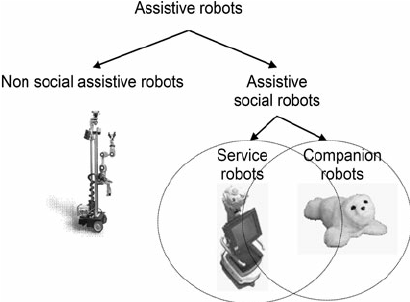
\includegraphics[scale=0.45]{gambar/robots-category.png}
	\caption{Pengategorian \emph{assistive robots} menurut Heerink et al.}
	\label{fig:RobotsCategory}
\end{figure}

\emph{Socially Assistive Robots} (\emph{SARs}) merupakan adaptasi dari \emph{assistive technology} yang meliputi keseluruhan sistem robotika yang mampu memberikan bantuan kepada pengguna dalam bentuk interaksi sosial \citep{Seifer2005}.
Heerink et al. \citep{Heerink2010} mengategorikan riset terhadap \emph{SARs} menjadi dua kategori berbeda seperti pada gambar \ref{fig:RobotsCategory}.
Kategori pertama mencakup robot yang menawarkan bantuan fisik dan kognitif yang melakukan tugas sebagai pelayan, sedangkan kategori kedua mencakup robot dengan dukungan sosial yang melibatkan robot berjenis pendamping sebagai sahabat dan media untuk terapi.
Lebih lanjut Rich et al. \citep{Rich2009} menjelaskan \emph{SARs} mampu memberikan bantuan kepada pengguna dalam berbagai tingkatan seperti:
(a) mendukung kemampuan fungsional dan kognitif pengguna;
(b) menawarkan pengguna kesempatan untuk meningkatkan partisipasi sosial dan kesehatan psikologis;
(c) menyediakan pemantauan jarak jauh dan berkelanjutan atas status kesehatan pengguna;
dan (d) membina pengguna untuk memfasilitasi promosi perilaku sehat dan pencapaian tujuan yang berhubungan dengan kesehatan.

\subsection{\emph{ROS 2}}

\emph{Robot Operating System} (\emph{ROS}) \citep{Quigley2009} merupakan kumpulan dari \emph{libraries}, \emph{drivers}, dan \emph{tools} yang mempermudah pengembangan sistem pada robot.
\emph{ROS} memiliki \emph{command tool} seperti \emph{Linux}, sistem komunikasi antar proses, dan berbagai macam \emph{packages} yang berhubungan dengan pengembangan sistem pada robot.
Proses yang dieksekusi pada \emph{ROS} disebut sebagai \emph{Node}, komunikasi antar proses yang dimiliki menggunakan model \emph{Publish}/\emph{Subscribe}, dan data komunikasi yang dikirimkan disebut sebagai \emph{Topic}.
Suatu proses \emph{Publisher} mampu mem-\emph{publish} satu maupun lebih \emph{Topic} dan proses-proses lain yang men-\emph{subscribe} suatu \emph{Topic} bisa memperoleh isi dari \emph{Topic} tersebut.

Generasi kedua dari \emph{Robot Operating System}, \emph{ROS 2}, merupakan kelanjutan dari \emph{ROS} yang mengusung reliabilitas dan performa untuk penggunaan \emph{real-time} sembari masih mendukung keunggulan yang dimiliki oleh \emph{ROS} sebelumnya \citep{Maruyama2016}.
Untuk memenuhi kebutuhan reliabilitas dan performa untuk penggunaan \emph{real-time} tersebut, \emph{ROS 2} menggunakan \emph{Data Distribution Service} (\emph{DDS}) \citep{Castellote2003} \citep{Schlesselman2004}, standar industri untuk sistem komunikasi \emph{real-time} dan \emph{end-to-end middleware}, yang menggantikan sistem komunikasi antar proses yang dimiliki \emph{ROS} sebelumnya.

\subsection{\emph{Gazebo}}

\emph{Gazebo} \citep{Koenig2004} merupakan bagian dari \emph{Player Project} \citep{Gerkey2003} yang memungkinkan sebuah simulasi robot dan aplikasi sensor berjalan di lingkungan \emph{indoor} maupun \emph{outdoor} tiga dimensi.
\emph{Gazebo} memiliki arsitektur \emph{Client}/\emph{Server} dan model \emph{Publish}/\emph{Subscribe} untuk sistem komunikasi antar prosesnya.
Setiap objek simulasi di \emph{Gazebo} dapat diasosiasikan dengan satu maupun lebih \emph{controllers} yang akan memproses perintah untuk mengatur dan menentukan keadaan dari suatu objek.
Data yang dihasilkan oleh suatu \emph{controller} akan dikirim ke \emph{shared memory} menggunakan \emph{Gazebo interfaces} (\emph{ifaces}).
Nantinya \emph{ifaces} dari proses-proses lain dapat membaca data tersebut pada \emph{shared memory}, sehingga memungkinkan komunikasi antar proses antara \emph{software} yang mengontrol robot dan \emph{Gazebo}, terlepas dari bahasa pemrograman maupun perangkat komputer yang digunakan.